\chapter{三维空间上的线性MARS算法}
在二维的界面追踪中,
基于MARS理论框架的iPAM方法\cite{zhang14:iPAM}和
cubic MARS方法\cite{zhang18:cubicMARS}将界面追踪的尺度和流相模拟的尺度$h$分离,
要求两者满足关系,
\begin{equation}
h_L=r_{\alpha}h^{\alpha}.
\end{equation}
这种设计使得用户可以根据实际情况来设置应用程序中$r_{\alpha}$以及$\alpha$的值,
为数值模拟带来了很大的灵活性.
当选择$r_{\alpha}=1$, $\alpha=1$时,iPAM方法的界面追踪精度是二阶的,
这样的选择使得计算成本相对降低,适用于界面追踪在物理过程中不起决定性作用的情况.
当选择$\alpha=1,\frac{3}{2}, 2$时,cubic MARS方法的界面追踪精度分别达到了四、六、八阶,
这是由于相较于iPAM, cubic MARS用了一组三次样条来近似流相的边界曲线,
cubic MARS方法的高精度为多相流的研究提供了更多的可能性.


在二维情况中除了上界$h_L$以外,
我们还设置了相邻示踪点之间距离的下界$r_{\mathsf{tiny}}h_L$. 
这样做的原因有三个,
第一,示踪点之间的距离下界$r_{\mathsf{tiny}}h_L$保证了示踪点的数量不会无限地增长,
使得示踪点的数量存在上界,
从而使得整个算法的数值稳定性更高,同时也提高了计算效率.
第二,当两个示踪点之间的距离过小时,
在求解近似曲面的样条时会出现许多鲁棒性问题\cite{kettner08:_class_examp_of_robus_probl},
设置距离下界可以有效地排除这些问题.
第三,通过下界的设置使得各个相邻示踪点之间的距离大致均匀,
从而提高了示踪点标记使用的效率,节省了计算的储存量.


在二维情况下由于流体的边界是曲线,
因此在界面追踪的过程中,我们只需要考虑控制示踪点之间的距离.
而在三维情况下,
边界则变成了曲面,
很自然我们需要控制三角形的面积大小,
然而只控制三角形的边长并不能够保证三角形的面积不会过小.
三角形的面积过小就意味着一定面积的曲面上,
三角形的面积和示踪点的数目会没有上界,
这会加大计算储存量,对算法的效率也有很大的影响.
因此在三维的线性MARS算法中,
我们在边长限制$[r_{\mathsf{tiny}}h_L,h_L]$的基础上
增加了一个面积下界$r_a=r_{\mathsf{tiny}}$,
当三角形面积小于$\frac{r_a\cdot h_L^2}{2}$时,
我们考虑删除该三角形.
边长的上下界以及面积下界保证了三角剖分中的最小角,
\begin{equation}
\label{eq:minAngle}
\theta_{\mathrm{min}}>\arcsin (r_a).
\end{equation}
这保证了界面的三角剖分具有较好的正则性,
也为今后的样条曲面插值做了准备.

\section{linear MARS算法定义}
 \begin{figure}
 	\label{fig:linMARS}
	\centering
	\subfigure[向前追踪边界 ${\cal M}^n$上的示踪点]{
		\includegraphics[width=0.45\linewidth]{pst/linearMARS1}
	}
	\hfill
	\subfigure[通过增加示踪点来使得三角形的边长都小于上界$h_L$]{
		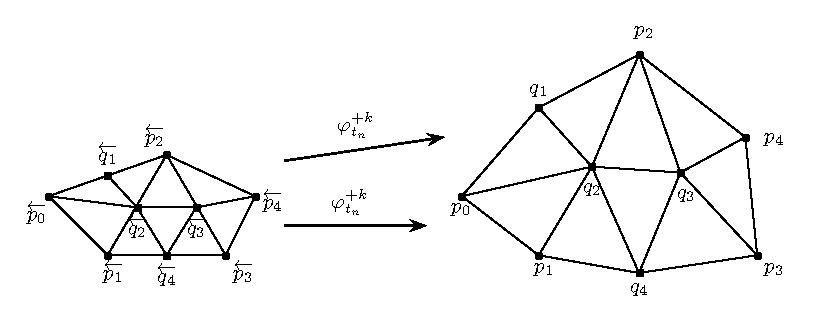
\includegraphics[width=0.45\linewidth]{pst/linearMARS2}
	}
	
	\subfigure[删除面积小于$\frac{r_ah_L^2}{2}$且超过两条边小于$r_{\mathsf{tiny}}h_L$的三角形]{
		\includegraphics[width=0.45\linewidth]{pst/linearMARS3}
	}
	\hfill
	\subfigure[删除面积小于$\frac{r_ah_L^2}{2}$且只有一条边小于$r_{\mathsf{tiny}}h_L$的三角形]{
		\includegraphics[width=0.45\linewidth]{pst/linearMARS4}
	}
	
	\subfigure[通过换边法优化三角形网格]{
		\includegraphics[width=0.45\linewidth]{pst/linearMARS5}
	}
	\hfill
	\subfigure[删除面积小于$\frac{r_ah_L^2}{2}$且三边均标准的三角形]{
		\includegraphics[width=0.45\linewidth]{pst/linearMARS6}
	}
	\caption[linear MARS方法的前三个步骤演示]{linear MARS方法的前三个步骤:
		在子图(a)中,
		界面 $\partial{\cal M}^n$上的示踪点被流映射$\varphi_{t_n}^{+k}$离散地映射到了像上.
		在子图(b)中,
		当 三角剖分中存在大于 $h_L$的边长的时候,
		通过添加示踪点来使得三角剖分的边长小于边长上界$h_L$.
		在子图 (c)中, 
		$\triangle_{p_1 p_2 p_3}$的面积小于  $\frac{r_ah_L^2}{2}$,
		且三边均小于$r_{\mathsf{tiny}}h_L.$ 
		将三角形 $\triangle_{p_1 p_2 p_3}$ 和另外三个与它共享一条边的三角形从三角剖分信息中删除,
		将顶点$p_1,p_2,p_3$用其重心来替换.
		在子图 (d)中,
		$\triangle_{p_1 p_2 p_3}$的面积小于$\frac{r_ah_L^2}{2}$, 
		其中$\overline{p_1 p_2}$小于边长下界,
		将$\overline{p_1 p_2}$ 缩成一个点,
		用其中点来替换点$p_1$, $p_2$ ,
		并把$\overline{p_1 p_2}$所在的两个三角形从三角剖分信息中删除.
		在子图 (e)中,
		三角形 $\triangle_{p_1 p_2 p_3}$的面积小于$\frac{r_ah_L^2}{2}$,
		通过换边法优化三角网格.
		在子图(f)中,
		换边法无法优化网格,
		则将三角形最小边用其中点替换.
	}
\end{figure}

\begin{defn}
	\label{defn:linMARS}
	在三维linear MARS方法中,
	用户需给出初始时刻流相边界的三角剖分信息作为其近似,
	并指定三角剖分中三角形边长界限$[r_\mathsf{tiny}h_L,h_L]$和三角形面积的下界$r_a$.
	三维linear MARS方法在每一个时间步$[t_n,t_n+k]$内,
	输入$\partial\mathcal{M}(t_n)$的三角剖分信息,
	通过以下步骤得到流相边界在$t_n+k$时刻的三角剖分信息作为对$\partial \mathcal{M}(t_{n+1})$的近似.

	\begin{enumerate}[{(linMARS}-1)]
		\setlength{\itemsep}{0pt}
		\setlength{\parsep}{0pt}
		\setlength{\parskip}{0pt}
		\item 对$\partial\mathcal{M}(t_n)$上的示踪点由流速场$\mathbf{u}$求解常微分方程
	           	     $\frac{\text{d}\mathbf{x}}{\text{d}t}=\mathbf{u}$
		             得到这些示踪点在$t_n+k$时刻的位置,记为$\{p_j\}$.
		\item 检查每一个三角形,若$\triangle_{p_i p_j p_k}$存在一条或一条以上的边大于上界$h_L$, 
		\begin{enumerate}[(a)]
			\item 在$\partial\mathcal{M}^n$上定位$\triangle_{p_i p_j p_k}$的顶点原像$\overleftarrow{p_i},
			             \overleftarrow{p_j}, \overleftarrow{p_k}$, 将大于上界$h_L$的边用其中点平分,并将这些中点标记为新的示踪点;
			\item 添加新边,用$\overleftarrow{p_i}, \overleftarrow{p_j}, \overleftarrow{p_k}$
			             和新的示踪点构建一个新的局部三角剖分;
			\item 用新的局部三角剖分来替代$\triangle_{p_i p_j p_k}$;
			\item 对于这些新的示踪点由流速场$\mathbf{u}$求解常微分方程
			            $\frac{\text{d}\mathbf{x}}{\text{d}t}=\mathbf{u}$得到这些新的示踪点
			            在$t_n+k$时刻的位置
			            并加入到顶点序列$\{p_j\}$中.
		\end{enumerate}
		重复以上步骤直到所有边长都不大于上界$h_L$.
		\item 检查每个三角形,若$\triangle_{p_i p_j p_k}$的面积小于$\frac{r_a \cdot h_L^2}{2}$
		             且满足删除条件(删除条件见下文分析),
		\begin{enumerate}
			\item 若三角形$\triangle_{p_i p_j p_k}$中有两条或以上的边小于$r_{\mathsf{tiny}}h_L$,
			             将该三角形缩成一个点;
			\item 若三角形$\triangle_{p_i p_j p_k}$仅有一边小于$r_{\mathsf{tiny}}h_L$,
			             将该边缩成一个点;
			\item 若三角形$\triangle_{p_i p_j p_k}$三条边都符合标准,用换边法优化网格,
			             若无法优化则将三角形的最小边缩成一个点.
		\end{enumerate}
	\item 得到一个新的三角剖分信息来近似$t_{n+1}$时刻的流相边界.
	\end{enumerate}
\end{defn}
在linear MARS中,显然(linMARS-3)中的三种处理方式
涵盖了所有面积小于$\frac{r_ah_L^2}{2}$且满足删除条件的三角形.


在定义\ref{defn:linMARS}中,
对于三角形的删除,我们还设置了可删除的限制条件.
如图3.2(a),
$p_0$是由$\triangle_{p_0 p_2 p_1}, \triangle_{p_0 p_3 p_2 }, \triangle_{p_0 p_1 p_3}$的交点,
$\triangle_{p_1 p_2 p_4}$与$\triangle_{p_0 p_2 p_1}$相交于$\overline{p_1 p_2}$,
当$\overline{p_1 p_2}$小于下界时,
若将其用中点$q$代替,
$\triangle_{p_0 p_1 p_3}$与$\triangle_{p_0 p_2 p_3}$的交是$\triangle_{p_0 q p_3}$,
网格不再是单纯复形,此时我们拒绝删除操作.
另外,当流向的局部变得极细的时候,为了保持其流相特征,
其附近的三角形可能很小,
如图3.2(b),
当$\overline{p_1p_2}$小于边长下界时,
若将其缩成一个点,三棱柱截断,流相的拓扑结构的改变.
由此可见,设置删除操作的限制是十分必要的.

\begin{figure}[htb]
	\label{fig:noDelete}
	\centering
	\subfigure[尖点附近的网格信息示例]{
		\includegraphics[width=0.4\linewidth]{images/111}
	}
	\hfill
	\subfigure[流相极细处的网格信息示例]{
		\includegraphics[width=0.4\linewidth]{images/333}
	}
	\caption{不满足删除条件的网格示例}
\end{figure}

假设$T$是所定位的要进行删除操作的三角形,
$T$是流相界面三角剖分的子复形,
对其进行删除操作所影响的区域很显然是在$\mathrm{star}(T)$范围内的,
因此在删除操作前,我们需要对$\mathrm{star}(T)$进行分析.
设集合$A=\{\mathbf{a}_1,\cdots,\mathbf{a}_i\}$是star$M$中所有三角形法向的集合,
定义$\mathrm{star}(T)$的平面最大夹角,
\begin{equation}
\label{defn:maxTheta}
\theta_T=\arccos(\min_{\textbf{a}_j\in A}|\mathbf{a}_T\cdot\mathbf{a}_j |).
\end{equation}
$\mathbf{a}_T$是三角形$T$的单位法向,
$\theta_T$直观地反应了$\mathrm{star}(T)$局部平面的平整程度,
当$\mathrm{star}(T)$趋于平整的时候,我们允许进行删除操作,
用户也可以自行指定$\cos\theta_T$的下界来限制删除操作的进行.
\begin{prop}
	linear MARS方法中流相界面的三角剖分在每一个时间步都是一个2-复形.
\end{prop}

\begin{proof}
(linMARS-2)中的(b)操作,保证了局部三角剖分是一个2-复形,
而(a)操作保证对每个局部三角剖分之间的公共边的处理一致,
因此(linMARS-2)保持了界面三角剖分是一个2-复形.
(linMARS-3)中的删除操作影响仅在$\mathrm{star}(T)$范围内,
分别考虑$\mathrm{star}(T)$内的2-单形和1-单形.
以图\ref{fig:linMARS}(d)的操作为例,
2-单形$\triangle_{p_1 p_2 p_3}$有三个1维面
$\overline{p_1 p_2}, \overline{p_1 p_3}, \overline{p_2 p_3}$.
首先考虑与$\triangle_{p_1 p_2 p_3}$的交集分别是1维面
$\overline{p_1 p_2}, \overline{p_1 p_3}, \overline{p_2 p_3}$的三个2-单形,
记作$\triangle_{p_1 p_2 p_4}, \triangle_{p_2 p_3 p_5}, \triangle_{p_1 p_3 p_6}$.
其中,2-单形$\triangle_{p_1 p_2 p_4}$塌缩成了1-单形.
又因$\triangle_{p_1 p_2 p_3}$塌缩成了一个1-单形$\overline{p_3 q}$,
$\triangle_{p_2 p_3 p_5}$的1维面$\overline{p_2 p_3}$
及$\triangle_{p_1 p_3 p_6}$的1维面$\overline{p_1 p_3}$均被$\overline{p_3 q}$替换,
因此$\overline{p_3 q}$是$\triangle_{p_1 p_3 p_6}$和$\triangle_{p_2 p_3 p_5}$的交.
当且仅当$\triangle_{p_2 p_3 p_5}$与$\triangle_{p_1 p_3 p_6}$的交
不包含除$\overline{p_3 q}$以外的1维面时,
网格保持是一个2-复形,而上述删除限制保证了这一条件.


对于$\mathrm{star}(T)$范围内的1-单形,
三个1-单形$\overline{p_1 p_2}, \overline{p_1 p_3}, \overline{p_2 p_3}$
塌缩成了一个1-单形$\overline{p_3 q}$,
$\triangle_{p_1 p_2 p_4}$与$\triangle_{p_1 p_2 p_3}$的交是$\overline{p_1 p_2}$,
又$\overline{p_1 p_2}$塌缩成了0-单形,
$\overline{p_4 q}$与$\overline{p_3 q}$相交于点$q$.
 而其他任意一个1-单形与$\overline{p_3 q}$的交集要么是空集,
 要么是单个0维面.
 假设存在一个1-单形$\overline{p_i p_j}$,
 其与$\overline{p_3 q}$的交集包含了两个或以上的点,
 则$\overline{p_i p_j}$至少与$\overline{p_1 p_2}, \overline{p_1 p_3}, \overline{p_2 p_3}$
 中的某一个1-单形的交集包含了两个或者以上的点,
 这与初始网格是一个单纯复形相矛盾,
 因此$\mathrm{star}(T)$范围内的任意两个1-单形都满足它们的交不是空集就是单个0维面.

综上,再由定义\ref{defn:simplex}可得
linear MARS中流相界面的三角剖分在每一个时间步都是一个2-复形.
\end{proof}

\section{linear MARS误差分析}
\begin{prop}
	\label{prop:error}
	(linear MARS方法的收敛性)三维空间上的linear MARS
	   在1-范数\eqref{defn:error}下是$2\alpha$精度的,
	    若其满足以下条件:
	\begin{enumerate}[(a)]
		\item 离散流映射$\mathring{ \phi}$在时间积分上至少是$2\alpha$阶精度的;
		\item 时间步长满足$k=O(h)$;
		\item $h_L=r_{\alpha} h^{\alpha}$满足$r_{\alpha}=O(1)$且$\alpha\geq 1$.
	\end{enumerate}
\end{prop}
\begin{proof}	
	根据\eqref{defn:accuracy}可得,
	linMARS的整体误差是多个单一误差的线性累加,
	因此我们只需对每个算子分别进行误差估计.
	通过(linMARS-2)和假设(b)和(c),在任意时间步,
	若界面上的两个相邻的顶点之间的最大距离为$h_{\mathrm{max}}=O(h^{\alpha})=O(k^{\alpha})$.
	根据误差定义\eqref{eq:geomError}得通过添加三角剖分中边的中点来作为新的示踪点不会增加误差,
	因此$E^{\textsf{AUG}}=0$.
	接下来证明任意时间步两个相邻点之间的最大距离$h_{\mathrm{max}}=O(h^{\alpha})$
	以及调整算子$\chi$带来的误差$E^{\textsf{ADJ}}=O(k^{2\alpha})$即可.
	
	
	由(linMARS-2)保证了当时相邻两个示踪点之间的距离最大为$h_L$. 
	(linMARS-3)中的删除操作会造成三角形顶点的偏移,
	从而造成相邻示踪点之间的距离扩大.
	但显然删除操作所造成的影响范围仅在删除三角形的星形范围内.
	当三角形面积小于$\frac{r_ah_L^2}{2}$时进行删除操作,
	所以在\ref{defn:linMARS}(f)中缩成点的边的长度有,
	\begin{equation*}
	l\leq\sqrt{\frac{h_L^2}{4}+(r_ah_L)^2}\leq(\frac{1}{2}+r_a)h_L.
	\end{equation*}
因此顶点的偏移距离最多为$\frac{1}{2}(\frac{1}{2}+r_a)h_L<h_L$,可得任意时间步内,
两个相邻示踪点之间的最大距离不超过$2h_L$,即$h_{\mathrm{max}}=O(h^{\alpha})$.
下证调整算子$\chi$带来的误差$E^{\textsf{ADJ}}=O(k^{2\alpha})$.

	 \begin{figure}[htbp]
		\label{fig:noDelete}
		\centering
			\includegraphics[width=0.7\linewidth]{images/error}
		\caption{调整算子误差分析图}
	\end{figure}
	
	如图3.3所示,记$\triangle_{p_i p_{i+1} p_{i+2}}$的星形为$\mathrm{star}(T)$,
	记调整之后的$\overline{p_i q}$的星形为$\mathrm{star}(E)$.
	调整算子在对于$\triangle_{p_i p_{i+1} p_{i+2}}$进行删除时,
	仅移动了$\triangle_{p_i p_{i+1} p_{i+2}}$上的两个顶点,
	而$\mathrm{star}(T)$边界上的顶点以及边并没有进行任何调整,
	因而$\mathrm{star}(T)$和$\mathrm{star}(E)$形成了一个闭合曲面,
	由\eqref{defn:error}可知调整算子所带来的误差是该闭合曲面所包围的体积.
	又由隐函数定理可得,一定存在一个投影平面,
	使得$\mathrm{star}(T)$和$\mathrm{star}(E)$均可以作为该投影平面上的连续二次函数,
	分别记为$F_1$和$F_2$,且$F_1$和$F_2$有相同的投影区域$D$.
	$\mathrm{star}(T)$和$\mathrm{star}(E)$形成的闭合曲面所包围的体积是,
	\begin{equation*}
	\int\int_{D}|F_1-F_2|\mathrm{d}\sigma.
	\end{equation*}
	由积分中值定理可得在$D$内,至少存在一点$(\varepsilon,\mu)$,使得
	\begin{eqnarray}
	\int\int_{D}|F_1-F_2|\mathrm{d}\sigma=|F_1(\varepsilon,\mu)-F_2(\varepsilon,\mu)|\cdot\sigma_0.
	\end{eqnarray}
	其中$\sigma_0$是该投影区域$D$的面积,是$O(h_L^2)$,
	因此该闭合曲面所包围的体积最大应是$O(h_L^4)$.
	由于在界面上的示踪点的数量为$O(\frac{1}{h_L^2})$,
	因而在每一个时间步执行次操作的次数最多是$O(\frac{1}{h_L^2})$,
	故调整算子$\chi$对与静态半代数集$\mathcal{P}$造成的误差是$O(h_L^2)$.
	当$\mathcal{P}$上存在$C_1$不连续点时,
	上述闭合曲面所包围的体积可能达到$O(h_L^3)$,
	但Sard定理指出$C_1$不连续的点至多只有常数个,
	因此上述对调整算子所带来的误差分析依然成立.
	
	
	综上所述,调整算子$\chi$对静态半代数集$\mathcal{P}$所造成的误差是$O(h_L^2)$. 
	由\eqref{lem:ADJerror}可得每个时间步都有$\|\varepsilon_n^{\textsf{ADJ}}\|=O(kh_L^2)$.
	因此,存在一个$c_k=O(1)$使得
	\begin{equation}
	E^{\textsf{ADJ}}\leq c_k\sum_{j-1}^n\|\varepsilon_j^{\textsf{ADJ}}\|=O(h^2).
	\end{equation}
	最后根据推论\eqref{cor:errorbound}命题得证.
\end{proof}